\documentclass[../ut-dissertation.tex]{subfiles}

\begin{document}
../commands.tex
\chapter{Introduction}
\begin{quote}
\textit{Nam cum pictor praecogitat quae facturus est, habet quidem in
intellectu sed nondum intelligit esse quod nondum fecit.}

-- Anselm of Canterbury~\cite{anselm}
\end{quote}
In the eleventh century, Anselm of Canterbury wrote what has since
come to be known as the ontological argument for the existence of
God~\cite{anselm}.  Anselm's argument was based on the assumption that
all ideas, or more specifically, all thoughts originate either from
perceptions of the outside world or from images formed within the
imagination.  From this he provides an argument for the existence of
a divine being.  The research presented here follows this same
epistemological assumption to a much less trivial end.
Instead of proving divine influence, the present work shall attempt to
measure the influence present in the written works of less divine beings.

The basic assumption made about text documents is the same assumption
that Anselm made about the origin of thoughts.  Every word, phrase,
sentence, paragraph, and theme in a document must come from one of two
sources.  Either the author created the thought from within their own
mind, and as such this counts as a literary contribution, or the
author could have transferred ideas from some outside source.  These
sources can take on many forms.  In the case of academic writing, the
author is likely to have been influenced primarily by the various
books and papers that they have read over the course of their
research.  Of course, another form of influence is a coauthor (though
in the case of academic literature, coauthors are almost always
explicitly stated.)  Of course, the influence over the text in a paper
is not constrained merely to the literature that the author has cited,
but is ultimately a reflection of an author's entire life experience
and background.  In the case of literary writing, such as a novel or
play, a reasonable assumption is that an author is influenced by other
works within their genre as well as by the society in which they live.

Given that every written document is influenced by at least a small
set of outside documents, the present work attempts to model and
quantify this influence by separating documents into a set of factors
and then searching for common factors among the documents.  The
desired result has two parts.  First, a weight is assigned to each
factor indicating its importance in the target work.  Second, the
factors themselves should carry enough semantic meaning to identify
the ideas and elements of style which have been transferred from a
source document to a target document.  Thus, the goal of the present
work is to identify influencing factors and to quantify the influence
they exert on a target document.

The usefulness of such a measurement should be readily apparent to
anyone working in any academic field.  In modern research, the
performance of participants is rooted in an attempt to measure that
person's influence over their chosen field.  Traditional approaches to
this problem involve counting citations over a specific window of time
~\cite{adler2009} while more modern approaches tend to involve some
document semantics~\cite{dietz2007, jiang2014}. Measuring
influence in a written document can also be applied in situations
where authorship is in question.  Given a corpus of works of confirmed
provenance, and a disputed document, influence modeling can identify
the possible influence of each author.  Thus textual influence
modeling can be used to answer the question of authorship where it is
disputed, or could potentially be used to identify plagiarized
passages.


\section{Modeling Influence}
At a high level, an influence model identifies elements that appear to
have been incorporated into a target document from a source document.
These elements are numerous, and are generally perceived on an
intuitive level.  For example, they could include elements of style,
topics, phrases, or ideas.  A human reader seems to be able to
identify these elements on an intuitive level, as can be seen readily
whenever a reader says one author ``sounds like'' another.  This
operation is also in effect when tracing ideas through written
academic literature.  In either case, the text of a target document
along with its corpus of cited documents seems to provide sufficient
evidence to identify potential sources of influence in the target
document.

The chief problem with an intuitive model such as the one outlined in
the previous paragraph is that it is highly subjective.  Every
conclusion reached by human scholars in such a system must appeal to
intuition and logic, and so determining the strength of any perceived
relationships present in the corpus presents a difficult challenge.
In recent years, the emerging field of computational stylistics has
offered several techniques for quantifying these elements of style
which can serve as markers of influence~\cite{bader2007, craig2009,
  burrows2017}.  In so much as it can, computational stylistics has
the principal goal of using textual evidence to answer the question of
authorship.  The current state of the art techniques for addressing
these questions rely upon statistical analysis of word frequencies
within documents~\cite{craig2009}.  The typical approach is to use a
set of ``marker words'' to determine the likelihood of an author's
contribution to a target document.  Those words that are more likely
to occur in the works of one author are ascribed to them if there is
sufficient statistical significance of the word's classifying power.
This current approach offers only a coarse level of determination.
Computational stylistic analysts can identify words that are more
likely to come from one author's work, and they in turn identify
whether that author appears to have contributed to a target document.
Thus the current techniques only inform the probability of an author's
contribution as a dichotomy.  Each potential author was either a
contributor, or they were not.  The objective of the model outlined in
this dissertation is to extend this model to include more detail.  As
opposed to determining whether an author has contributed to a target
work directly, this model assumes that influence is present in
multiple forms; the present model seeks to identify the strength of
influence, as well as to identify what those specific influences were.

\subsection{Tensors and Decompositions}
In order to analyze a document, it must first be quantified in some
way that allows for analysis.  The model discussed in this
dissertation represents documents using tensors.  The term tensor has
been broadly applied across multiple fields to describe several
different types of related objects.  For the purposes of factor
analysis, a tensor is simply an extension of matrices into a higher
number of modes. In tensor terminology a ``mode'' is a dimension along
which the tensor can be indexed.  A scalar is a mode zero tensor, a
vector is a mode one tensor, and a matrix is a mode two tensor.  When
the number of modes exceeds two, it is customary to refer to the array
simply as a tensor.  A detailed account of the tensor operations
performed by this model is given in the next chapter.  For a complete
treatment of tensors as they pertain to factor analysis, see Tamara
Kolda's tutorial~\cite{kolda2009}.


The underlying principle of tensor analysis is polyadic decomposition,
which was first described by Frank Hitchcock in
1927~\cite{hitchcock1927}.  When a tensor is expressed in polyadic
form, it is expressed as the sum of rank 1 tensors, which is usually
written as the outer product of vectors.  (This is also referred to as
the tensor product of vectors, which is in line with the geometric
interpretation of tensors as the outer product of vector spaces.)
Each polyadic factor in a tensor of $m$ modes is the tensor product of
$m$ vectors.  For example, given a 3-mode tensor $\tens{T} \in
\R^{I\times J \times K}$, its polyadic decomposition into $r$ factors
is a set of factors which satisfies
Equation~\ref{eq:polyadic_decomposition}.  For the sake of
convenience, the remainder of this discussion will assume a three
mode tensor, however everything discussed here can readily be extended
to any number of modes.

\begin{equation} \label{eq:polyadic_decomposition}
  \tens{T} \approx \dsum_{i=1}^{r} a_i \otimes b_i
  \otimes c_i
\end{equation}

The tensor, or outer,  product $a \otimes b$ used in
Equation~\ref{eq:polyadic_decomposition} results in a tensor where the
modes are the concatenation of the modes of $a$ and $b$.  For
instance, if $a$ and $b$ are vectors of size $i$ and $j$ respectively,
$a \otimes b$ results in a 2-mode tensor with dimensions $i x j$.  In
the case of building a 3-mode tensor, three vectors are needed, and
the elements of the product result are computed as in in
Equation~\ref{eq:tensor_product}. A graphical representation of this
product is showin in Figure~\ref{fig:tensor_product}.  Of note is
how each vector serves as scaling values for a mode.  
\begin{equation} \label{eq:tensor_product}
  \tens{T}_{ijk} = a_i b_j c_k
\end{equation}

\begin{figure}[p]%
  \centering
  \subfloat[Mode Vectors]{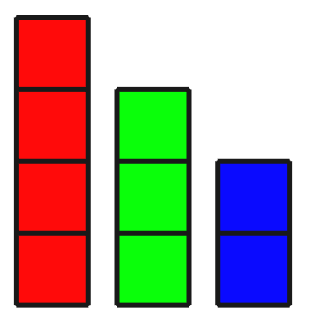
\includegraphics[width=1.5in]{diagrams/mode_vectors}}
  \qquad
  \subfloat[$a \otimes b$]{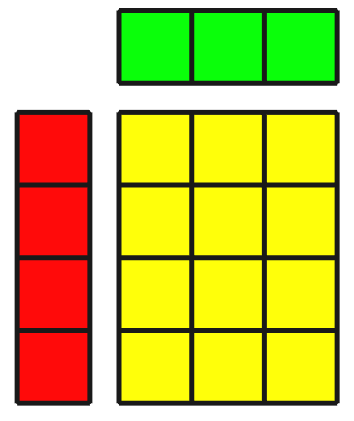
\includegraphics[width=1.5in]{diagrams/mode1_tns_mode2}}
  \qquad
  \subfloat[$a \otimes b \otimes c$]{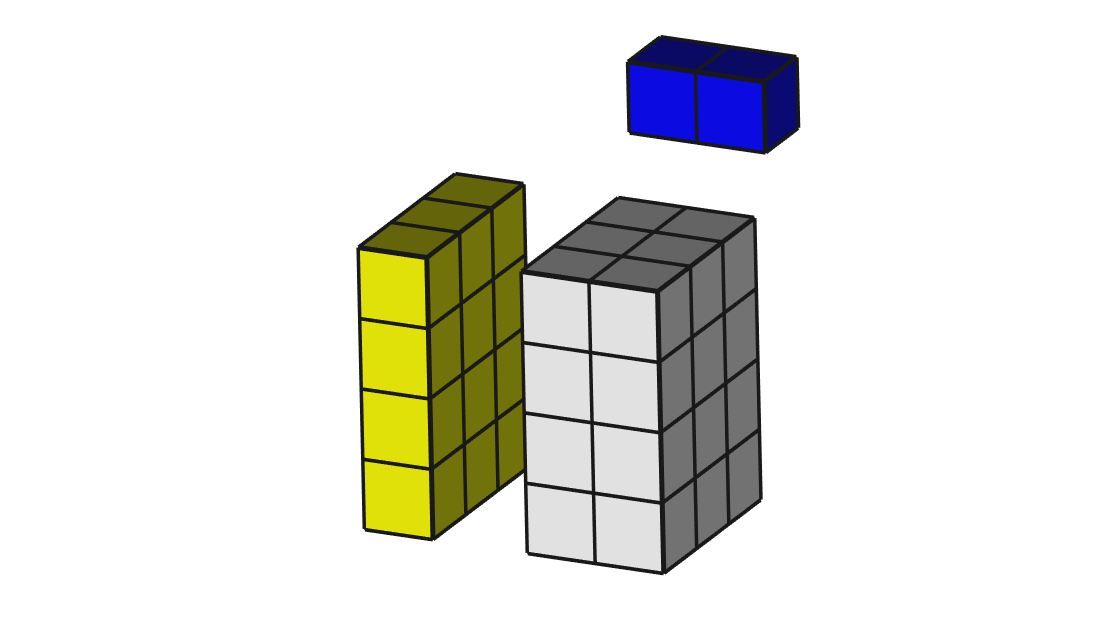
\includegraphics[width=1.5in]{diagrams/mode12_tns_mode3}}
  \caption{Tensor Product} \label{fig:tensor_product}
\end{figure}
\FloatBarrier

The notion of the tensor product also gives rise to the notion of
tensor rank.  Tensor rank is not the same as matrix rank, and is in
fact much more difficult to compute.  Perhaps the easiest way to
understand the notion of tensor rank is recursive.  A rank 1 tensor is
a tensor which can be constructed completely from the tensor product
of 1-mode tensors (vectors).  The tensor descibed in
Equation~\ref{eq:tensor_product} and
Figure~\ref{fig:tensor_product} is therefore a rank-1 tensor, as are
all the factors in the polyadic decomposition.  A tensor of general
rank $r$ is the result of adding $r$ rank-1 tensors together. The rank
of a tensor $\tens{T}$ is therefore defined as the minimum number of
rank-1 tensors needed to sum to $\tens{T}$.

Hitchcock's paper mainly presents the polyadic decomposition from a
purely mathematical perspective, with applications to studying tensor
invariants and tensor rank.  In fact, as later papers show, the
problem of determining the rank of a tensor is
NP-Complete~\cite{haastad1990}.  Polyadic decomposition began to see
other uses when it was rediscovered in 1970 by Richard
Harshman~\cite{harshman1970}, Douglas Carroll, and Jih-Jie
Chang~\cite{carroll1970}.  Harshman coins the term ``PARAFAC'', a
portmanteau of ``Parallel Factors'' while Carroll and Chang refer to
the model as ``CANDECOMP'' in placed of ``Canonical Decomposition''.
Both papers present the model as a means of studying psychological
data by treating the tensor factors as explanatory variables for the
variance in the tensor data.  In recent years, tensor analysis has
begun to take root in other fields such as chemometrics~\cite{bro1997}
and text mining~\cite{bader2007}.  In several modern treatments, the
polyadic decomposition is referred to as ``CPD'' or ``Canonical
Polyadic Decomposition''.  For the purposes of factor analysis,
factors are often normalized, without loss of
generality~\cite{bro1997, bader2007}, yielding the decomposition shown
in Equation~\ref{eq:polyadic_decomposition_normalized}.
\begin{equation} \label{eq:polyadic_decomposition_normalized}
  \tens{T} \approx \dsum_{i=1}^{r} \lambda_i a'_i
  \otimes b'_i \otimes c'_i
\end{equation}
Here $\lambda_i$ is a scalar where $\lambda_i = \mathrm{norm}(a_i
\otimes b_i \otimes c_i)$.  This is desirable because the factors in
this form are proportional profiles~\cite{harshman1970} with all of
the magnitude of the factor contained in $\lambda_i$.  As can be
clearly seen from Equation~\ref{eq:polyadic_decomposition_normalized},
$\lambda_i$ is also an expression of the influence that factor $i$
exerts over the tensor $\tens{T}$.  For this reason, factors are
typically expressed in order from largest $\lambda_i$ to the smallest
$\lambda_i$.  Thus these factor norms serve the same purpose as
eigenvalues in principal component analysis, or as singular values in
singular value decomposition.

In fact, the similarities between PCA, SVD, and CPD do not end with
the inclusion of weights!  Nor is it true that CPD is the only tensor
decomposition.  The closest competing decomposition is the Tucker
decomposition, first proposed in 1963 and fully formed in
1966~\cite{kolda2009}.  Given tensor $\tens{T}$, the Tucker
decomposition yields the factor matrices $\mat{
  A}\in\R^{I\times P}$, $\mat{ B} \in
\R^{J\times Q}$, and $\mat{ C}\in
\R^{K\times R}$.  The model also contains a so-called core
tensor $\tens{G} \in \R^{P\times Q \times R}$.  These
factors are fit to satisfy Equation~\ref{eq:tucker_decomposition},
where $\tens{G} \times_n \mat{M}$ is the $n$-mode product of
tensor $\tens{G}$ and matrix $\mat{M}$.  

\begin{equation}\label{eq:tucker_decomposition}
  \tens{T} \approx \tens{G} \times_1 \mat{A} \times_2 \mat{B} \times_3
  \mat{C}
\end{equation}

An element-wise version of the tucker decomposition is shown in
Equation~\ref{eq:tucker_decomposition_elements}.  For a complete
treatment of the $n$-mode tensor matrix product, see the Kolda
tutorial~\cite{kolda2009}.

\begin{equation}\label{eq:tucker_decomposition_elements}
  t_{ijk} \approx \dsum_{p=1}^P \dsum_{q=1}^Q \dsum_{r=1}^R
  g_{pqr}a_{ip}b_{jq}c_{kr}
\end{equation}

As was shown by Henk Kiers, the relationship between PCA, Tucker
decomposition, and CPD is hierarchical~\cite{kiers1991}.  While
Kiers's paper focuses on 3-way analysis, his results extend to any
number of modes.  Because a tensor can be unfolded along any dimension
to form a two dimensional matrix, it is always possible to use PCA to
find explanatory factors for tensor data.  In fact, Tucker-3 is a
constrained version of PCA.  The exact nature of these constraints is
beyond the scope of the present discussion, however they are a direct
result of the presence of the core tensor.  A simplified summary is
that the core tensor's dimensions predetermines the number of
factors to be discovered.  CPD, in turn, is a constrained variant of
the Tucker decomposition.  While the CPD is usually written without a
core tensor, it can be thought of as having an identity tensor as its
core.  The identity tensor is simply a tensor with ones along its
super-diagonal and zeros everywhere else.  (Or stated more formally,
an identity tensor is a tensor containing ones where $i_1 = i_2 =
\ldots =i_n$ for all $n$ modes and zeros in all other positions.)
Also, in CPD, $P=Q=R$ (and so on if there are more than three modes).
Tucker decomposition allows for each mode to have a different number
of factors, while CPD does not.  As can be expected, the more
constraints placed upon the explanatory model of the tensor comes at
the expense of quality of fit.  Hence, PCA will always provide the
best fit, Tucker will either be as good or worse than PCA, and CPD
will always be as good or worse than a Tucker model~\cite{kiers1991,
  bro1997}.

So then if the tensor decomposition models provide a worse fit, the
question becomes why are they important?  The answer lies in several
properties of the tensor decompositions.  First, tensor decompositions
retain the structure of the original data~\cite{harshman1970,
  kolda2009}.  Unfolding a tensor loses semantic information about the
variables being analyzed, and extracting intuitive semantics from the
resultant PCA model is difficult and usually
impossible~\cite{bro1997}.  Also, in the case of CPD, the factors are
unique under rotation so long as the number of factors extracted is
greater than or equal to the rank of the tensor~\cite{harshman1994}.
Another desirable property of the CPD is that it does not partition
space by hyper-surfaces.  Instead, it creates a sort of implicit set
of axes for factor separation by providing a proportional profile
along the tensor's basis~\cite{harshman1994}.  Thus if several tensors
of like dimensions are decomposed, their factors can be logically
thought of as existing within the same space.  This allows for
comparison among the factors to be carried out, unlike under PCA where
the factor space of each matrix is a projection into a new space,
making comparison of factors from disparate matrices difficult to
perform in a meaningful way.

In some instances of tensor analysis, it can be convenient to apply
additional constraints to the model.  The most common constraint
applied to CPD is a non-negativity constraint~\cite{liu2012sparse,
  bro1997, kolda2009}.  This is done for a variety of reasons, most
notably as a form of dimension reduction and when analyzing data which
are naturally predisposed to be non-negative.  In the model presented
in this dissertation, both outcomes are necessary.  First, the tensors
used in this model are extremely sparse, and so introducing negative
factors makes the search space for factors so large that fitting the
model becomes intractable.  Second, the tensors used in this model
represent frequency data, which means that negative values in factors
would have no valid semantic meaning.

\subsection{Representing Documents as Tensors}
The text documents to be analyzed are represented as a tensor by
dividing them into phrases of length $n$.  These phrases, commonly
referred to as $n$-grams, are counted and their frequencies are
entered into a tensor.  Each word in the corpus vocabulary is assigned
an index, and the tensors $n$ modes refer to these indexes.  For
example, suppose $n=3$.  The document tensor $\tens{D}$ would have
3 modes.  The entry $d_{ijk}$ refers to the frequency of the
$n$-gram consisting of words $i$, $j$, and $k$ from the corpus
vocabulary.  

The tensors produced by this encoding will be cubic.  Given a
vocabulary consisting of $v$ words, the resultant tensor will have $v$
indexes in each mode.  The tensor can represent the frequency of all
possible $n$-grams, and as such will be extremely sparse as very few
of these $n$-grams are likely to appear in a document.  When
decomposed into polyadic form, these tensors will yield sets of
related words as well as related $n$-grams that appear in the same
factors.  



\subsection{Modeling Influence}
The basic model applied to the document begins with the decomposition
of a document into its individual factor tensors.

\begin{equation} \label{eq:document_decomposition}
  \tens{D} = \sum \tens{F}_i 
\end{equation}
where $\tens{F}_i\in \set{F}$ is a factor of the tensor $\tens{D}$,
($\tens{F}_i=a_i \otimes b_i \otimes c_i$).  As has been previously
noted, the model becomes more expressive by separating out a
normalizing value $\lambda_i$ from each $f_i$.  Thus the decomposed
document becomes:
\begin{equation} \label{eq:document_decomposition_normal}
  \tens{D} = \sum \lambda_i \tens{F}'_i
\end{equation}
where $\tens{F}'_i=\frac{1}{|\tens{F}_i|} \tens{F}_i$ and
$\lambda_i = |\tens{F}_i|$.  This is desirable for two reasons.  Given
that all tensors within the corpus have the same dimensions, and that
all are decomposed using Non-Negative CPD, the factors occupy the same
type of space as the factors of other documents.  By normalizing them
into a proportional model of the document, the factors become directly
comparable irrespective of the magnitude of influence they exert in
their source document.

Let $\set{C}$ be a corpus of documents, encoded as tensors
$\tens{D}_j \in \set{C}$.  Let $\tens{D}_t$ be the target document to
be studied, and all other documents in $\set{S}=\set{C} - \tens{D}_t$
are treated as source documents for $\tens{D}_t$.  The goal of the
influence model is to ascribe the factors of $\tens{D}_t$ to a factor
from each source document $\tens{D}_s\in \set{S}$ and assign weights
to each of the source document influences. Each document in $\set{C}$
is decomposed as per Equation~\ref{eq:document_decomposition_normal}.
$\tens{D}_t$ is also decomposed into its components.  This produces
sets of factors $\set{F'}_s$ and $\Lambda_s$ for each source document
as well as $\set{F'}_t$ and $\Lambda_t$ for the target document.  By
measuring the similarity of each factor $f'_{t}\in\set{F'}_{t}$ and
source factors $f'_{s}\in \set{F'}_s$ in every $\set{F'}_s$, each
factor can be ascribed to a source document $\tens{D}_s$ or as being
original to $\tens{D}_t$.  Using the similarity measurements between
the $f'_t$ and $f'_s$ factors, each corresponding $f_t$ factor of
$\tens{D}_t$ is categorized as either belonging to one of several
sets: $F^s_t$ for all factors of $\tens{D}_t$ ascribed to some factor
of $\tens{D}_s$ and $F^n_t$ for all factors with no matching source.

For each of these factor sets, tensors can be formed by summing over
the set.  For every $\set{F}^s_t$, the tensor $\tens{F}^s_t$ is the
sum of all components of document $t$ ascribed to document $s$.  

Hence, the model of the target document can be rewritten:

\begin{equation} \label{eq:influence_factors}
  \tens{D}_t \approx \sum_{s=1}^{|\set{S}|} \tens{F}^s_t + \tens{F}^n_t
\end{equation}

Normalizing as in the previous equations, the target
document's model becomes:

\begin{equation} \label{eq:influence_factors_normalized}
  \tens{D}_t \approx \sum_{s=1}^{|\set{S}|} \lambda^s_t \tens{F}'^s_t +
  \lambda^n_t \tens{F}'^n_t
\end{equation}

These new factor tensors, which are no longer necessarily rank 1
tensors, contain the proportions of related $n$-grams, separated into
components according to their attributed source.  This comprises the
sought after semantic model of the document.  

Given these new factors, the influence of each document is extracted:

\begin{equation} \label{eq:document_lambda}
  \Lambda_t = (\lambda_1, \lambda_2, \ldots \lambda_{|S|}, \lambda_t)
\end{equation}

Weights for each document are then extracted as their proportion of
importance to the target document.

\begin{equation} \label{eq:document_weights}
  \set{W} = \dfrac{1}{\sum \Lambda_t} \Lambda_t
\end{equation}

Note that the weights from the source documents are not used.
Essentially, the only purpose the factors of the source documents
serve is to classify the factors of the target document.  Having
accomplished the classification step and constructed the model in
Equation~\ref{eq:influence_factors_normalized}, and extracted the
weights in Equation~\ref{eq:document_weights}, the target document has
been decomposed into a set of tensors which identify both the semantic
shape of each contribution and its corresponding weight.

\subsection{Summary of Influence Modeling Procedure}
Generating the above model can be subdivided into the following steps:

\begin{enumerate}
\item Encode each document in the corpus as a tensor.
\item Decompose each document using non-negative CPD.
\item Classify each factor of the target document $\tens{D}_t$ as
  either belonging to a source document or as an original contribution
  of the author.
\item Extract weights from each subset of factors to determine the
  influence of each class of factors.
\end{enumerate}

The details of how each of these steps is accomplished appears in the
next chapter of this dissertation.

\section{Related Work}
Much of the inspiration for frequency based analysis for authorship
detection comes from the work of John Burrows and Hugh
Craig~\cite{burrows2006, burrows2017, craig2009}.  In their papers,
Burrows and Craig utilize a variety of numerical techniques to explore
marker words, and they use frequencies of marker works coupled with
T-distribution sampling to provide an argument for attributing
authorship of disputed works.  They explore a variety of literary
works, ranging from poetry to Shakespeare's plays.  (Most of their
focus is on Elizabethan and Victorian era works.)  In all of these
works, the frequencies explored are based on single marker words, and
the words are extracted based on how unique they are to the authors in
question.

For $n$-gram classification, Noriaki's Kawamae's paper has shown that
$n$-grams are capable of building a generative topic model of a corpus
of documents~\cite{kawamae2016}.  Kawamae's work shows that a
combination of $n$-gram and word frequencies reveals information about
a corpus's structure, especially hierarchical information pertaining
to topics within the corpus.  Kawamae's model builds a tree with
probabilistic relationships which are then used to infer information
about the structure of a corpus, and shows that $n$-grams provide
a sufficient basis for modeling the transfer of ideas through a corpus.

Another related $n$-gram study was performed by Antonia, Craig, and
Elliott~\cite{antonia2014}.  In this paper, Antonia et. al. attempt to
reproduce marker word studies using $n$-gram frequencies in place of
word frequencies.  They were able to show that $n$-gram frequencies
are able to identify stylistic signatures of contributors to a text
document.  When $n=1$, their model is equivalent to marker words, and
as they increase $n$, they retest to determine how expressive the
model is.  They noted that there is no one length that seems to work
best in all cases when analyzing English language documents.  Their
results show that 1-gram, 2-gram, and 3-gram analysis tends to work
well, but when exploring longer phrases the power of the model drops
off.  Even in instances where 1-grams or 2-grams are best, 3-grams are
still a reasonable choice.  Based on this result, 3-grams will be used
in the tests in this dissertation.  The analysis performed in Antonia
et. al.'s work was conducted using delta and zeta tests as was
established in the standard marker word approach.  As such, only the
most frequent $n$-grams of each author were explored, and they were
only used as an evidentiary marker of an author's participation.  One
advantage that the analysis proposed in this dissertation has is that
it will account for all $n$-grams, and will explore how $n$-grams
relate to each other within the target document's structure.


\section{Outline of this Dissertation}
The rest of this dissertation is organized as follows.  First, there
is a chapter detailing the approach of building, fitting, and
evaluating the influence model.  Following the approach explanation
is an application which analyzes a conference paper and its sources.
The final chapter discusses the findings in the case
study as well as some notes for further application of this analysis
technique.

\end{document}
